\documentclass[border=6pt]{standalone}
\usepackage{mathptmx}
\usepackage[scaled=0.92]{helvet}
\usepackage[dvipsnames]{xcolor}
\usepackage{tikz}
\usetikzlibrary{positioning,fit,backgrounds,arrows.meta,calc,shapes.geometric,shadows}
\definecolor{caindigo}{HTML}{4F46E5}
\definecolor{cagreen}{HTML}{059669}
\definecolor{caorange}{HTML}{EA580C}
\definecolor{caslate}{HTML}{475569}
\definecolor{cared}{HTML}{DC2626}
\definecolor{caviolet}{HTML}{8B5CF6}
\definecolor{cabgindigo}{HTML}{EEF2FF}
\definecolor{cabggreen}{HTML}{ECFDF5}
\definecolor{cabgorange}{HTML}{FFF7ED}
\definecolor{cabgslate}{HTML}{F8FAFC}
\definecolor{cabgred}{HTML}{FEF2F2}
\definecolor{cabgviolet}{HTML}{F5F3FF}
\begin{document}
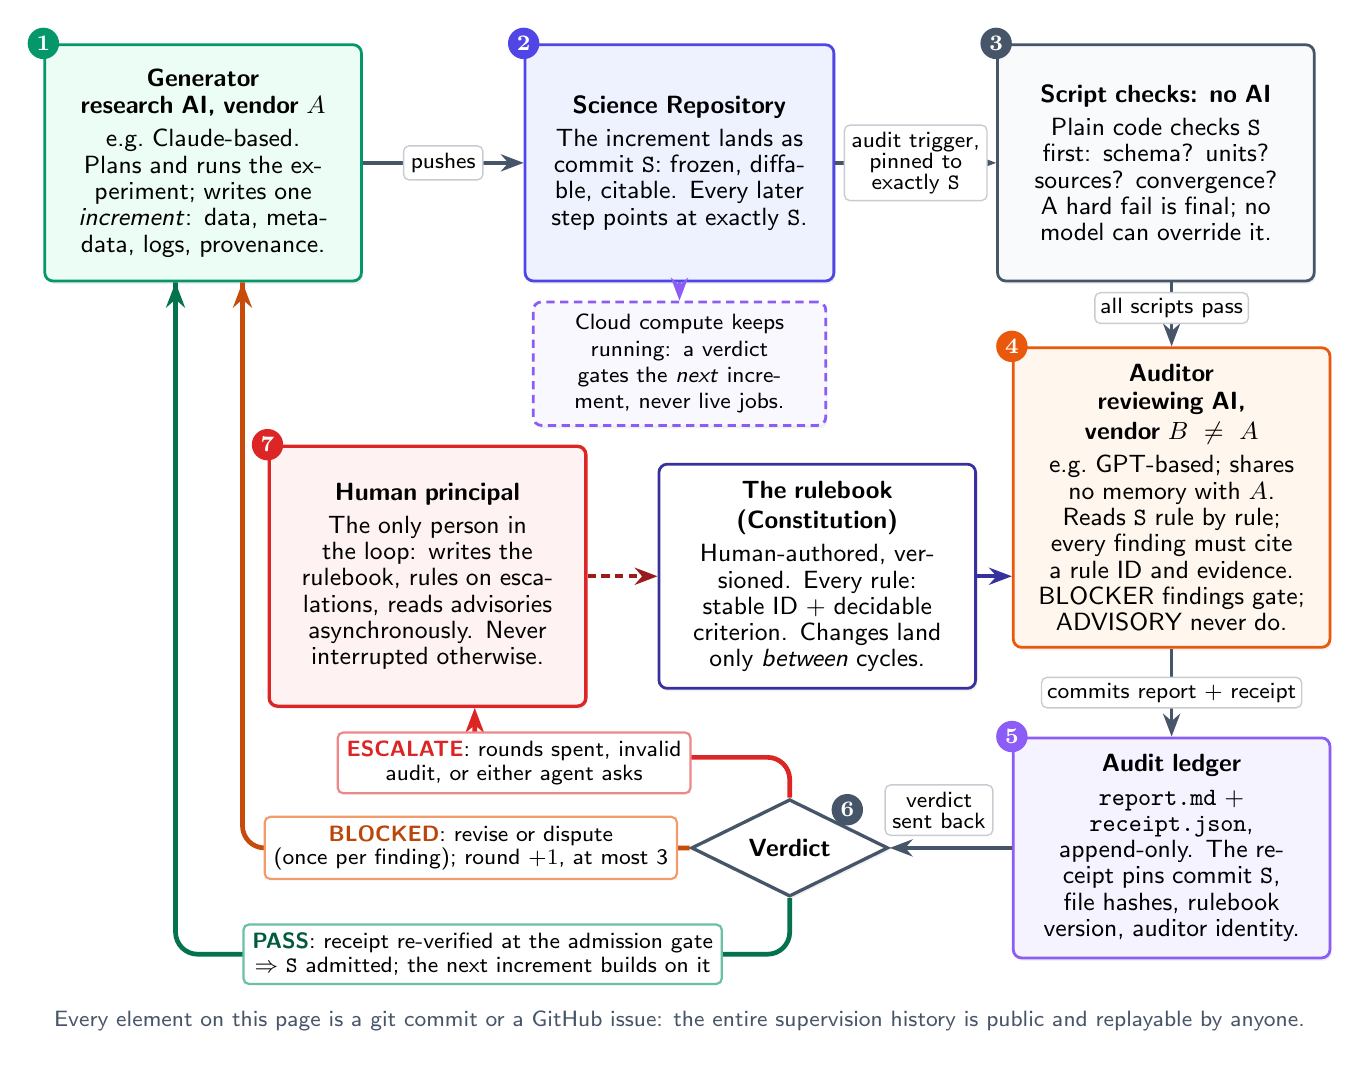
\begin{tikzpicture}[x=1cm, y=1cm,
  font=\footnotesize\sffamily,
  every shadow/.style={shadow xshift=0.6pt, shadow yshift=-1.1pt, opacity=0.12},
  box/.style={draw, rounded corners=3pt, align=center, inner sep=6pt, line width=1pt, drop shadow},
  gen/.style={box, draw=cagreen, fill=cabggreen, text width=36mm, minimum height=30mm},
  sci/.style={box, draw=caindigo, fill=cabgindigo, text width=35mm, minimum height=30mm},
  det/.style={box, draw=caslate, fill=cabgslate, text width=36mm, minimum height=30mm},
  aud/.style={box, draw=caorange, fill=cabgorange, text width=36mm},
  led/.style={box, draw=caviolet, fill=cabgviolet, text width=36mm},
  hum/.style={box, draw=cared, fill=cabgred, line width=1.2pt, text width=36mm, minimum height=33mm},
  con/.style={box, draw=caindigo!70!black, fill=white, text width=36mm},
  cmp/.style={box, draw=caviolet, fill=cabgviolet!60, densely dashed, text width=34mm, inner sep=4.5pt},
  ver/.style={draw=caslate, fill=white, diamond, aspect=1.45, align=center, inner sep=2.5pt, minimum width=25mm, line width=1.2pt, drop shadow},
  badge/.style={circle, text=white, inner sep=1.5pt, font=\bfseries\footnotesize},
  flow/.style={-{Stealth[length=2.9mm]}, line width=1.3pt, draw=caslate},
  fate/.style={-{Stealth[length=3.2mm]}, line width=1.7pt, rounded corners=8pt},
  lbl/.style={fill=white, align=center, inner sep=2.6pt, font=\footnotesize\sffamily, rounded corners=2pt, draw=caslate!30, line width=0.5pt},
  fatelbl/.style={lbl, line width=0.8pt, inner sep=3.2pt}
]
% ================= top row: produce, freeze, check =================
\node[gen] (gen) at (2.05,-1.50) {\small\textbf{Generator}\\[-1pt] \small\textbf{research AI, vendor $A$}\\[2.5pt] e.g.\ Claude-based. Plans and runs the experiment; writes one \emph{increment}: data, metadata, logs, provenance.};
\node[sci] (sci) at (8.10,-1.50) {\small\textbf{Science Repository}\\[2.5pt] The increment lands as commit \texttt{S}: frozen, diffable, citable. Every later step points at exactly \texttt{S}.};
\node[det] (dcl) at (14.15,-1.50) {\small\textbf{Script checks: no AI}\\[2.5pt] Plain code checks \texttt{S} first: schema? units? sources? convergence? A hard fail is final; no model can override it.};
% ================= middle band =================
\node[cmp] (cmp) at (8.10,-4.05) {Cloud compute keeps running: a verdict gates the \emph{next} increment, never live jobs.};
\node[hum] (hum) at (4.90,-6.75) {\small\textbf{Human principal}\\[2.5pt] The only person in the loop: writes the rulebook, rules on escalations, reads advisories asynchronously. Never interrupted otherwise.};
\node[con] (con) at (9.85,-6.75) {\small\textbf{The rulebook (Constitution)}\\[2.5pt] Human-authored, versioned. Every rule: stable ID $+$ decidable criterion. Changes land only \emph{between} cycles.};
\node[aud] (aur) at (14.35,-5.75) {\small\textbf{Auditor}\\[-1pt] \small\textbf{reviewing AI, vendor $B \neq A$}\\[2.5pt] e.g.\ GPT-based; shares no memory with $A$. Reads \texttt{S} rule by rule; every finding must cite a rule ID and evidence. BLOCKER findings gate; ADVISORY never do.};
% ================= bottom row =================
\node[ver] (ver) at (9.50,-10.20) {\small\textbf{Verdict}};
\node[led] (led) at (14.35,-10.20) {\small\textbf{Audit ledger}\\[2.5pt] \texttt{report.md} $+$ \texttt{receipt.json}, append-only. The receipt pins commit \texttt{S}, file hashes, rulebook version, auditor identity.};
% ================= badges =================
\node[badge, fill=cagreen]  at (gen.north west) {1};
\node[badge, fill=caindigo] at (sci.north west) {2};
\node[badge, fill=caslate]  at (dcl.north west) {3};
\node[badge, fill=caorange] at (aur.north west) {4};
\node[badge, fill=caviolet] at (led.north west) {5};
\node[badge, fill=caslate, anchor=south west] at ([xshift=-0.5mm, yshift=0.2mm]ver.north east) {6};
\node[badge, fill=cared]    at (hum.north west) {7};
% ================= forward flow =================
\draw[flow] (gen) -- node[lbl]{pushes} (sci);
\draw[flow] (sci) -- node[lbl]{audit trigger,\\[-2pt] pinned to\\[-2pt] exactly \texttt{S}} (dcl);
\draw[flow] (dcl.south -| aur.north) -- node[lbl, inner sep=2pt, yshift=0.8mm]{all scripts pass} (aur.north);
\draw[flow] (aur.south) -- node[lbl, inner sep=2pt]{commits report $+$ receipt} (led.north);
\draw[flow] (led.west) -- node[lbl, yshift=4.8mm, xshift=-1.5mm]{verdict\\[-2pt] sent back} (ver.east);
\draw[flow, densely dashed, draw=caviolet] (sci) -- (cmp);
\draw[flow, densely dashed, draw=cared!70!black] (hum) -- (con);
\draw[flow, draw=caindigo!70!black] (con.east) -- (con.east -| aur.west);
% ================= the three fates =================
\draw[fate, draw=cagreen!75!black] (ver.south) -- (9.50,-11.55) -- (1.70,-11.55) -- (1.70,-3.30) -- ([xshift=-3.5mm]gen.south);
\node[fatelbl, draw=cagreen!60] at (5.60,-11.55) {\textbf{\textcolor{cagreen!60!black}{PASS}}: receipt re-verified at the admission gate\\[-1pt] $\Rightarrow$ \texttt{S} admitted; the next increment builds on it};
\draw[fate, draw=caorange!85!black] (ver.west) -- (2.55,-10.20) -- (2.55,-3.30) -- ([xshift=5mm]gen.south);
\node[fatelbl, draw=caorange!60] at (5.45,-10.20) {\textbf{\textcolor{caorange!80!black}{BLOCKED}}: revise or dispute\\[-1pt] (once per finding); round ${+}1$, at most 3};
\draw[fate, draw=cared] (ver.north) -- (9.50,-9.05) -- (5.50,-9.05) -- ([xshift=6mm]hum.south);
\node[fatelbl, draw=cared!55] at (6.00,-9.12) {\textbf{\textcolor{cared}{ESCALATE}}: rounds spent, invalid\\[-1pt] audit, or either agent asks};
% ================= the ledger property, in words =================
\node[align=center, font=\footnotesize\sffamily, text=caslate, anchor=north] at (8.1,-12.15)
  {Every element on this page is a git commit or a GitHub issue: the entire supervision history is public and replayable by anyone.};
\end{tikzpicture}
\end{document}
